\chapter{Slip coefficient and Slip curve of Belt drive}
\section{Nomenclature}
\begin{tabular}[t]{lp{7cm}}
	$ a $ & center distance, $ mm $\\
	$ f $ & coefficient of friction\\
	$ d $ & diameter, $ mm $\\
	$ F_0 $ & initial tension, $ N $\\
	$ F_{ms} $ & friction force, $ N $\\
	$ F_t $ & tangential force, $ N $\\ 
	$ g $ & gravitational acceleration at sea level, $ m/s^2 $\\
	$ h_f $ & distance between outer sides of the belt after applying load $ Q $, $ mm $\\
	$ h_i $ & distance between outer sides of the belt before applying load $ Q $, $ mm $\\	
\end{tabular}
\begin{tabular}[t]{lp{7cm}}
	$ n $ & rotational speed, $ rpm $\\
	$ Q $ & load, $ kg\cdot F $\\
	$ \alpha $ & wrap angle, $ ^{\circ} $\\
	$ \beta $ & slack angle due to load $ Q $, $ \unit{^{\circ}} $\\
	$ \Delta h $ & difference between $ h_i $ and $ h_f $, $ \unit{mm} $\\
	$ \phi $ & drag coefficient\\
	$ \phi_{crit} $ & critical drag coefficient\\
	$ \bar{\xi} $ & average slip coefficient\\
	$ \tilde{\xi} $ & relative slip coefficient\\
	$ \xi $ & slip coefficient\\	
	$ _1 $ & subscript for driving pulley\\
	$ _2 $ & subscript for driven pulley\\
\end{tabular}
\section{Aim}
\begin{enumerate}
	\item Investigating on the slip phenomenon of belt drive.
	\item $ \tilde{\xi} $ and $ \xi $ determination.
	\item Determining $ F_0 $.
	\item Drawing slip curve - load diagram.
\end{enumerate}

\section{Technical rules on safety}
Students must comply with the technical rules on safety in the laboratory.

\section{Conducting and dealing with experimental results}
\subsection{Determine the parameters for the experimental model}
	\begin{itemize}
		\item Diameters of the pulley:\\
		$ d_1 = 67.8\unit{mm} $\\
		$ d_2 = 165\unit{mm} $
		\item Belt type: flat belt.
		\item Rotational speed: see table (\ref{dataexp1}).
		\item Contact angles:\\
			$ \alpha_1 = 180 - 57\times\dfrac{d_2-d_1}{a} \approx 162.3^{\circ}$\\
			 $ \alpha_2 = 180 + 57\times\dfrac{d_2-d_1}{a} \approx 197.6^{\circ}$
		\item Initial tension:\\
			$ h_i = 124\unit{(mm)}$, $ h_f = 94\unit{(mm)} $, $ Q = 4.1\unit{(kg\cdot F)} $\\
			$ \Delta_h=|h_f-f_i|=30\unit{(mm)} $, $ \beta=\arctan\dfrac{2\Delta_h}{a} \approx 10.78^{\circ}$\\
			$ F_0 = \dfrac{Qg}{2\sin\beta} \approx 107.48\unit{(N)}$

		\item Tangential force: see table (\ref{dataexp1}).
	\end{itemize}
\subsection{Measure and deal with the measured results of $ F_0 $}
\subsection{Measure and deal with the measured results in order to determine the $ \tilde{\xi} $ and $ \phi $.}
Filling out the measured results in table \ref{dataexp1} and calculate the coefficients. Using the formulas $ \xi=1-\dfrac{d_2n_2}{d_1n_1} $ and $ \phi=\dfrac{F_t}{2F_0} $, we obtain the following table:
\begin{table}[ht]
	\centering
	\renewcommand{\arraystretch}{1.5}
	\rowcolors{3}{}{lightgray!20}
	\begin{tabular}{crrrrrr}\toprule
		\multirow{2}{*}{No.} &\md{$ F_0$} & \md{$ n_1 $} & \md{$ n_2 $} & \md{$ \xi $} & \md{$ F_t $} & \md{$ \phi $}\\
		& \md{$ \unit{(N)} $} & \md{$ \unit{(rpm)} $} & \md{$ \unit{(rpm)} $} & & \md{$ \unit{(N)} $} & \\
		\midrule
		1 & 107.48 & 283.62 & 114.04 & 0.018 & 3.1 & 0.014\\
		2 & 107.48 & 330.47 & 133.35 & 0.018 & 8.8 & 0.041\\
		3 & 107.48 & 273.83 & 110.27 & 0.02 & 14.4 & 0.067\\
		4 & 107.48 & 307.52 & 123.71 & 0.021 & 20.2 & 0.094\\
		5 & 107.48 & 354.42 & 142.43 & 0.022 & 22.1 & 0.103\\\bottomrule
	\end{tabular}
	\caption{Experimental results of the slip coefficient}
	\label{dataexp1}
\end{table}\\
Averaging the values of $ \xi $ yields $ \bar{\xi} \approx 0.0198$
\subsection{Establish a graph of slip curve}
From the data above, we can approximate the best fitted line through the data points (assuming linearity since $ \phi $ does not reach critical value)
\begin{figure}[ht]
	\centering
	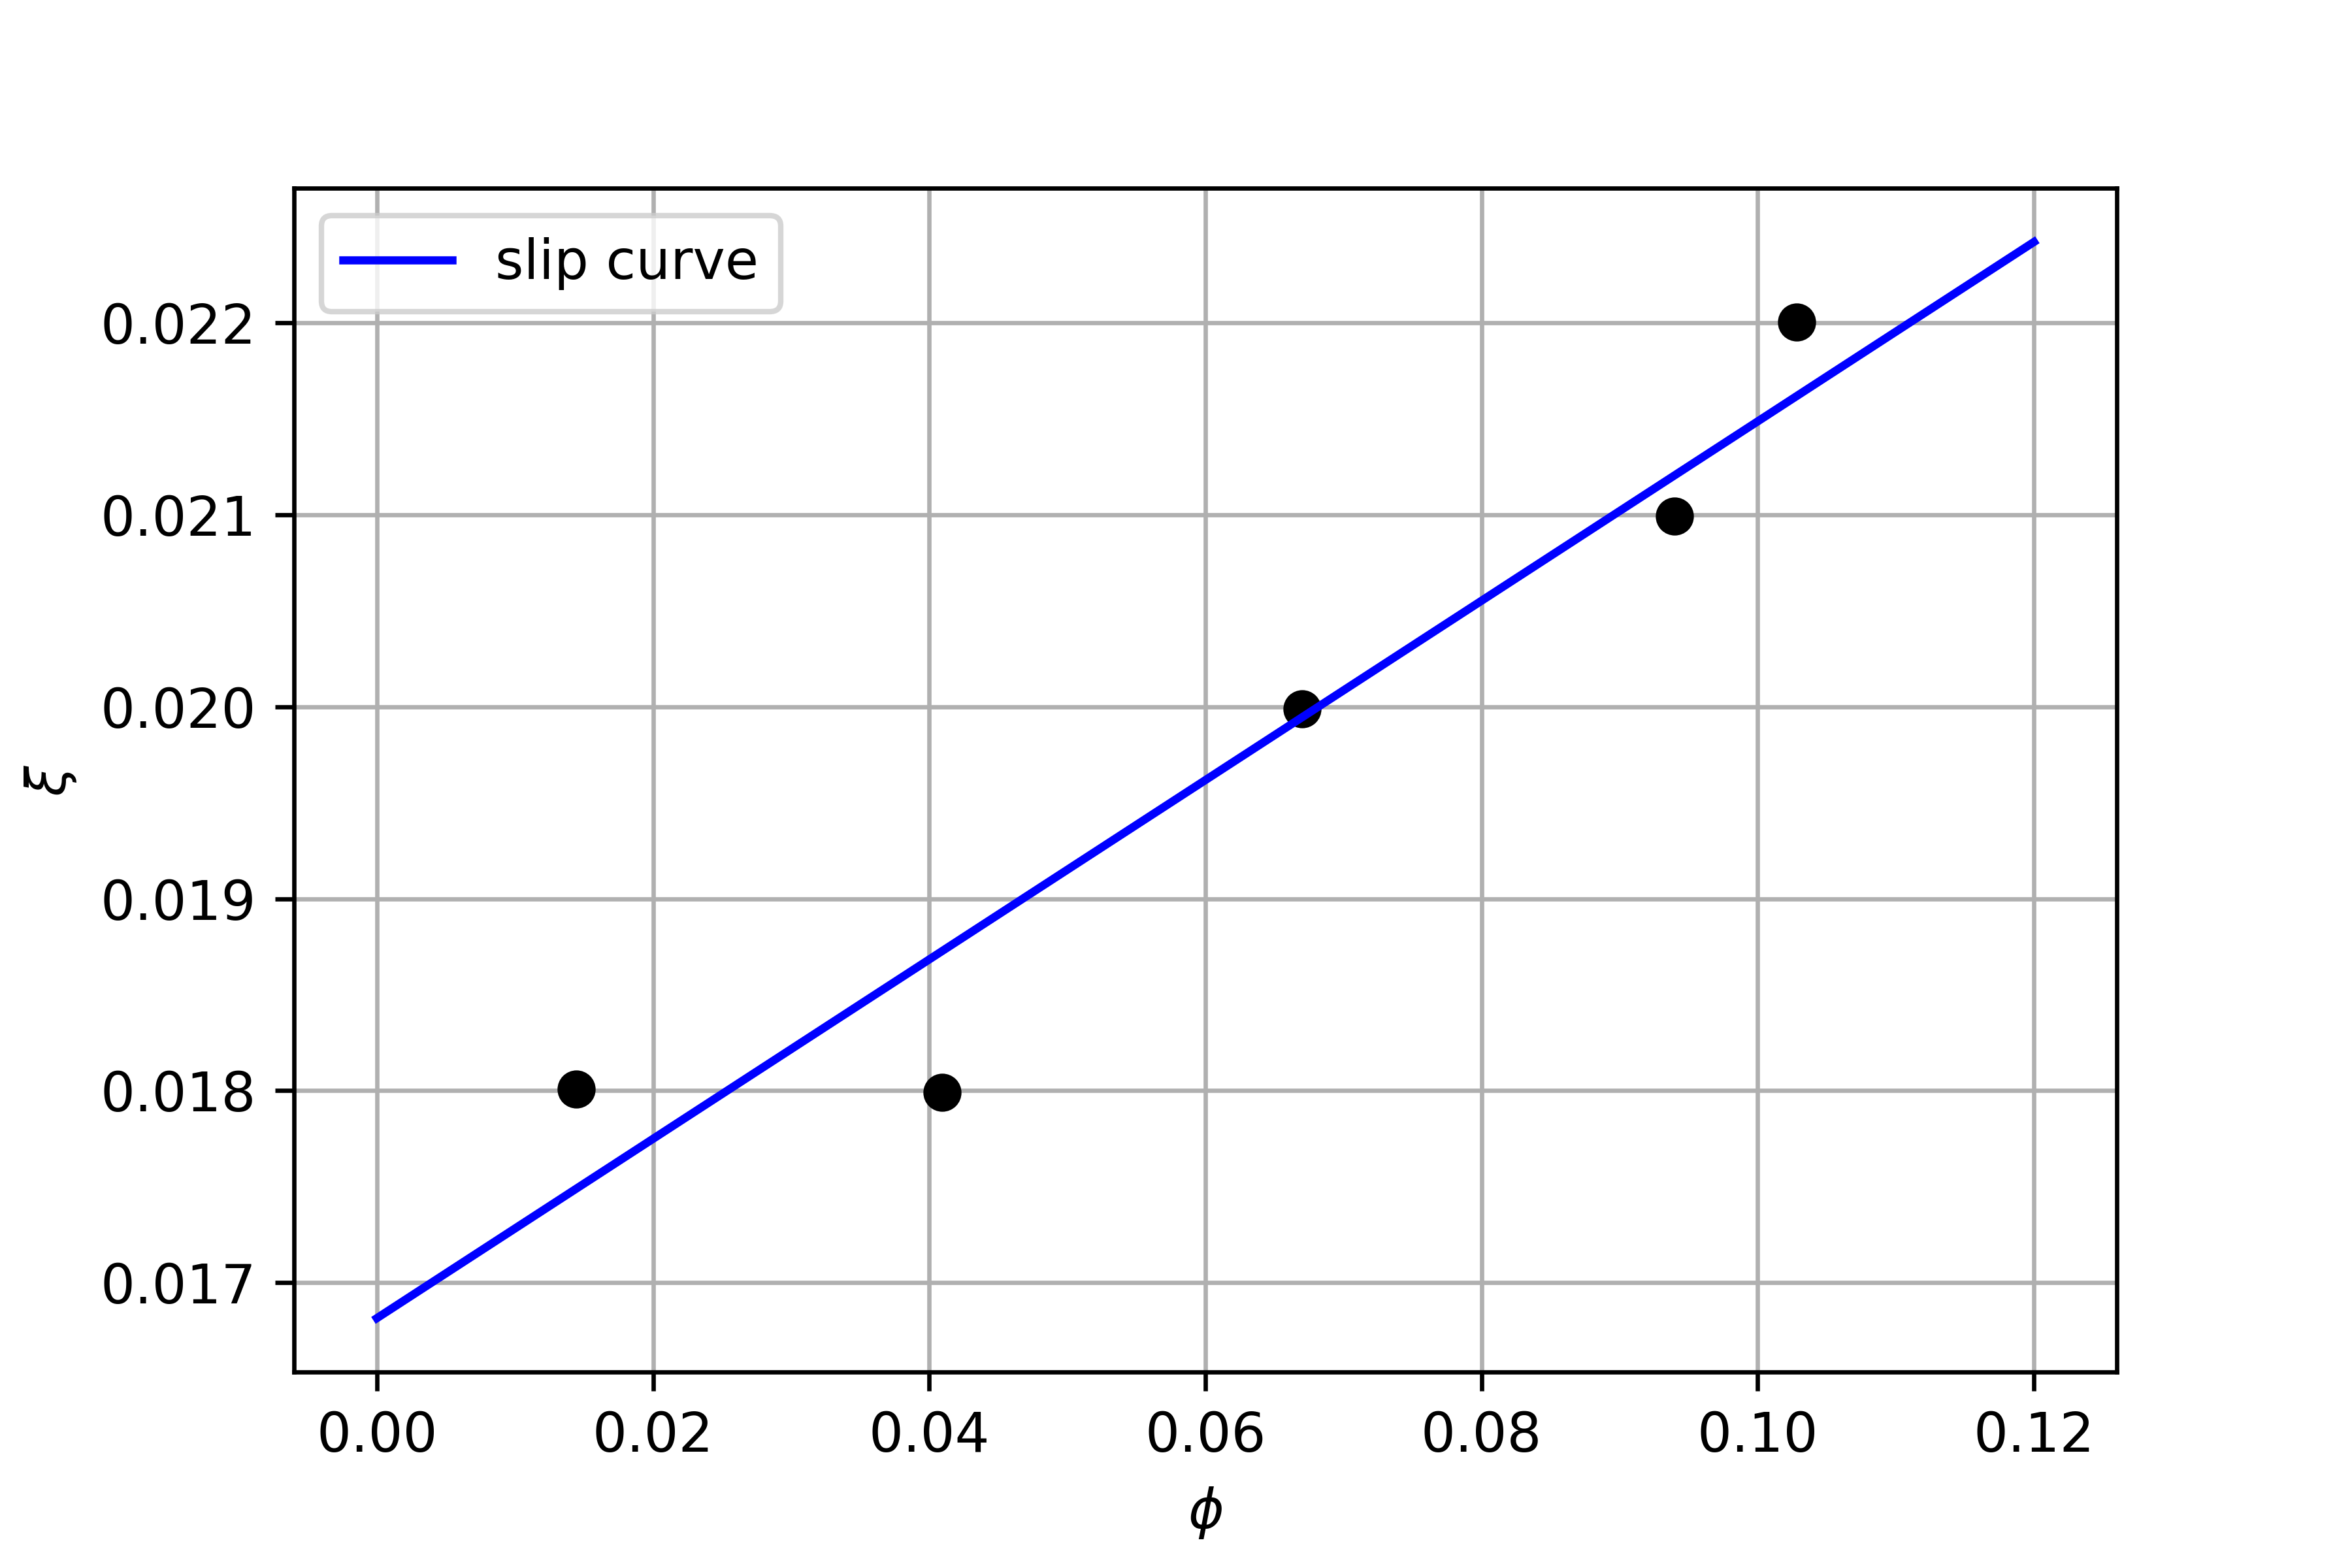
\includegraphics{Exp1.png}
	\caption{The clip curve is established by the experimental data.}
\end{figure}
\newpage

\section{Discussion and conclusions}
In summary:
\begin{itemize}
	\item Slip coefficient from experiment is in allowable range ($ 0.01\div0.02 $).
	\item The slip curve is in agreement with theory (error is smaller than $ 5\% $). Since $ \phi $ does not exceed critical value (the motor is frequency-controlled), we can safely assume linearity for the curve.
	\item Possible errors:
	\begin{itemize}
		\item manually measure dimensions in the kit.
		\item rounding.
		\item incorrect reading of rotational speeds.
	\end{itemize}
	\item The slip coefficient and slip curve is considerably accurate due to reliable instrument
\end{itemize}
\section{Review questions}
\begin{enumerate}
	\item Define the types of slip in the belt drive.
	\item The method determining the slip coefficient in the belt drive.
	\item  The relationship between $ F_t $ and $ F_0 $
	\item Present the formula determining $ \phi $ and the $ \phi_{crit} $ of the kinds of belt drives.
\end{enumerate}